\documentclass[11pt]{article}
\usepackage{geometry, titlesec}
\usepackage[parfill]{parskip}
\usepackage[italicdiff]{physics}
\usepackage{amsfonts, amsthm}
\usepackage[cm]{fullpage}
\usepackage{fancyhdr}
\usepackage{enumitem}
\usepackage{xcolor, soul}
\usepackage{graphicx}
\usepackage[export]{adjustbox}
\usepackage{siunitx}
%\allowdisplaybreaks

\renewcommand{\thesubsection}{\thesection.\alph{subsection}}
\setenumerate[1]{label={(\alph*)}}

\makeatletter
\renewcommand*\env@cases[1][1.2]{%
  \let\@ifnextchar\new@ifnextchar
  \left\lbrace
  \def\arraystretch{#1}%
  \array{@{}l@{\quad}l@{}}%
}
\makeatother
 
\renewcommand{\footrulewidth}{.2pt}
%\setlist[enumerate]{leftmargin=*}
\pagestyle{fancy}
\fancyhf{}
\lhead{Physics 132-B}
\chead{\textbf{Discussion 6 Problems}}
\rhead{A--De Discussion}
\setlength{\headheight}{11pt}
\setlength{\headsep}{11pt}
\setlength{\footskip}{24pt}
\lfoot{\today}
\rfoot{\thepage}

\titleformat{\subsection}[runin]{\normalfont\large\bfseries}{\thesubsection}{1em}{}
\newcommand{\refeq}[1]{(\ref{#1})}

\newcommand{\beq}{\begin{equation*}}
\newcommand{\eeq}{\end{equation*}}

\newcommand{\beqn}{\begin{equation}}
\newcommand{\eeqn}{\end{equation}}

\newcommand{\blg}{\begin{align*}}
\newcommand{\elg}{\end{align*}}


\newenvironment{statement}
{
%    \color{gray}
    \ignorespaces
}
{
%    \smallskip
}

\newenvironment{problem}
{
%    \color{darkgray}
    \ignorespaces
}

\newenvironment{solution}
{
    \paragraph{Solution.}
    \ignorespaces
}
{
    \bigskip
}

\renewcommand{\vec}[1]{\mathbf{#1}}


\begin{document}
	


\paragraph{Question 24.2}
\begin{problem}
	Suppose several different parallel-plate capacitors are charged up by a constant-voltage source.  Thinking of the actual movement and position of the charges on an atomic level, why does it make sense that the capacitances are proportional to the areas of the plates?  Why does it makes sense that the capacitances are \emph{inversely} proportional to the distance between the plates?
\end{problem}

\vfill

\paragraph{Question 24.20}
\begin{problem}
	A conductor is an extreme case of a dielectric, since if an electric field is applied to a conductor, charges are free to move within the conductor to set up ``induced charges.''  What is the dielectric constant of a perfect conductor?  Explain your reasoning.
\end{problem}

\vfill

\paragraph{Question 25.17}
\begin{problem}
	The energy that can be extracted from a storage battery is always less than the energy that goes into is while it is being charged.  Why?
\end{problem}

\vfill
\clearpage

\begin{minipage}[l]{0.75\textwidth}
\paragraph{Question 25.14}
\begin{problem}
	A light bulb glows because it has resistance.  The brightness of a light bulb increases with the electrical power dissipated in the bulb. \medskip
	\begin{enumerate}
		\item In the circuit shown in \textbf{Fig.~Q25.14(a)}, the two bulbs $A$ and $B$ are identical.  Compared to bulb $A$, does bulb $B$ glow more brightly, just as brightly, or less brightly?  Explain your reasoning. \medskip
		\item Bulb $B$ is removed from the circuit and the circuit is completed as shown in \textbf{Fig.~Q25.14(b)}.  Compared to the brightness of bulb $A$ in \textbf{Fig.~Q25.14(a)}, does bulb $A$ now glow more brightly, just as brightly, or less brightly?  Explain your reasoning.
	\end{enumerate}
\end{problem}
\end{minipage}%
\hspace{0.05\textwidth}%
\begin{minipage}{0.2\textwidth}
\center 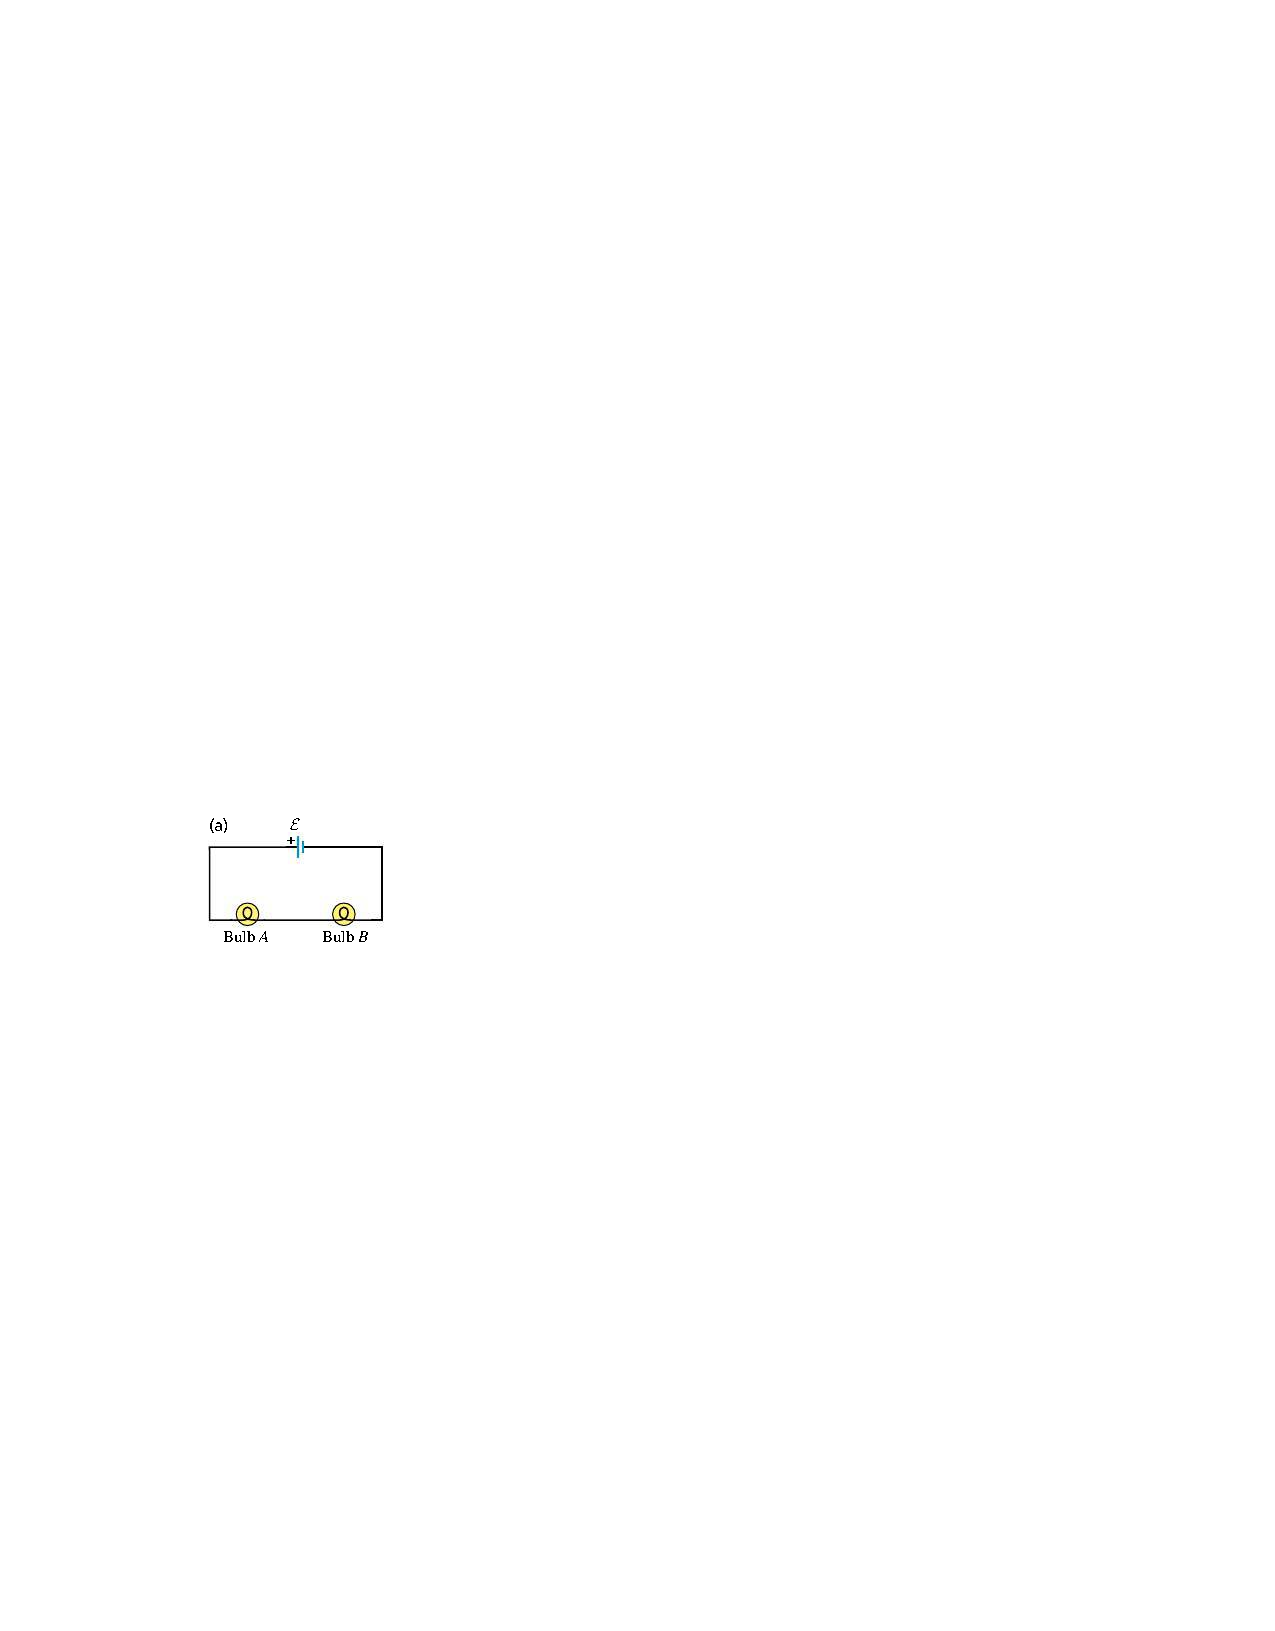
\includegraphics{Q25-14a} \\
\center 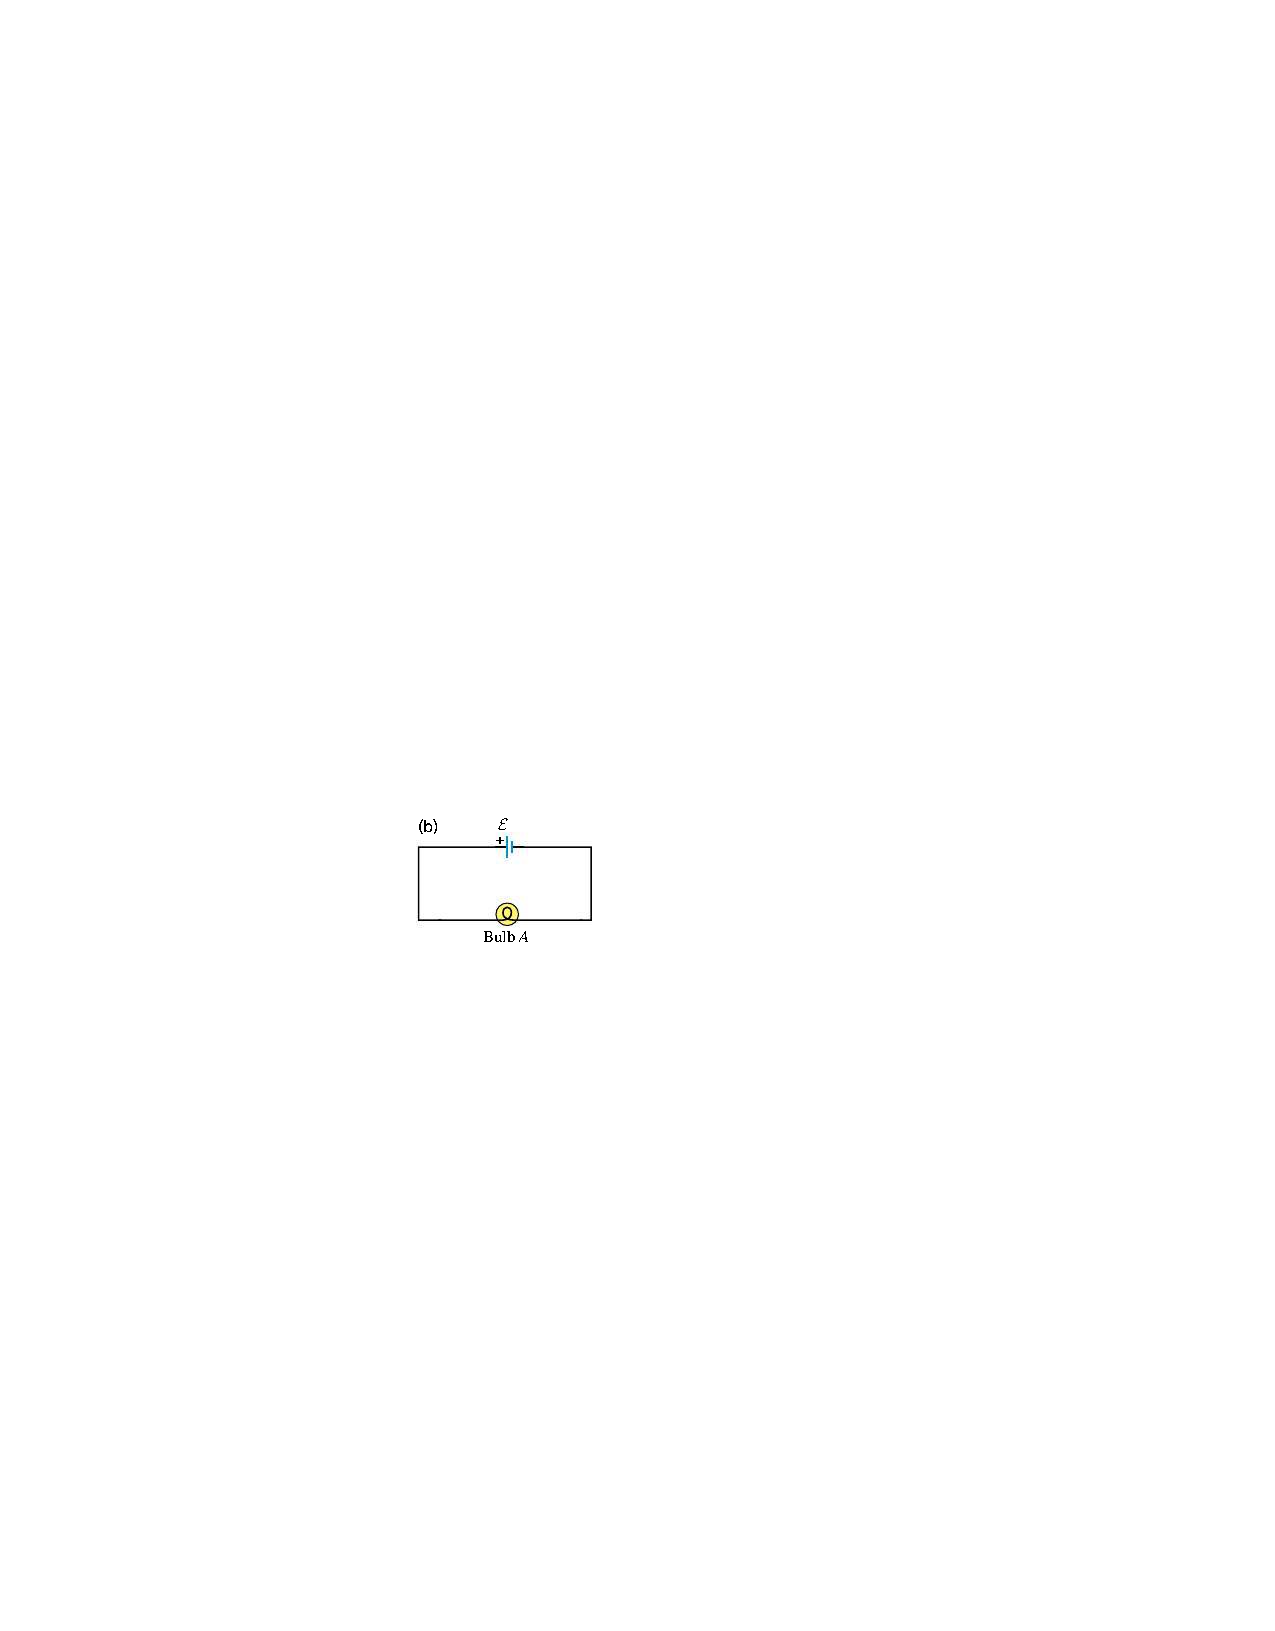
\includegraphics{Q25-14b}
\center \textbf{Figure Q25.14}
\end{minipage}

\vfill

\begin{minipage}[l]{0.7\textwidth}
\paragraph{Question 26.9}
\begin{problem}
	A light bulb is connected in the circuit shown in \textbf{Fig.~Q26.9}.  If we close the switch $S$, does the bulb's brightness increase, decrease, or stay the same?  Why?
\end{problem}
\end{minipage}%
\hspace{0.05\textwidth}%
\begin{minipage}{0.25\textwidth}
\center 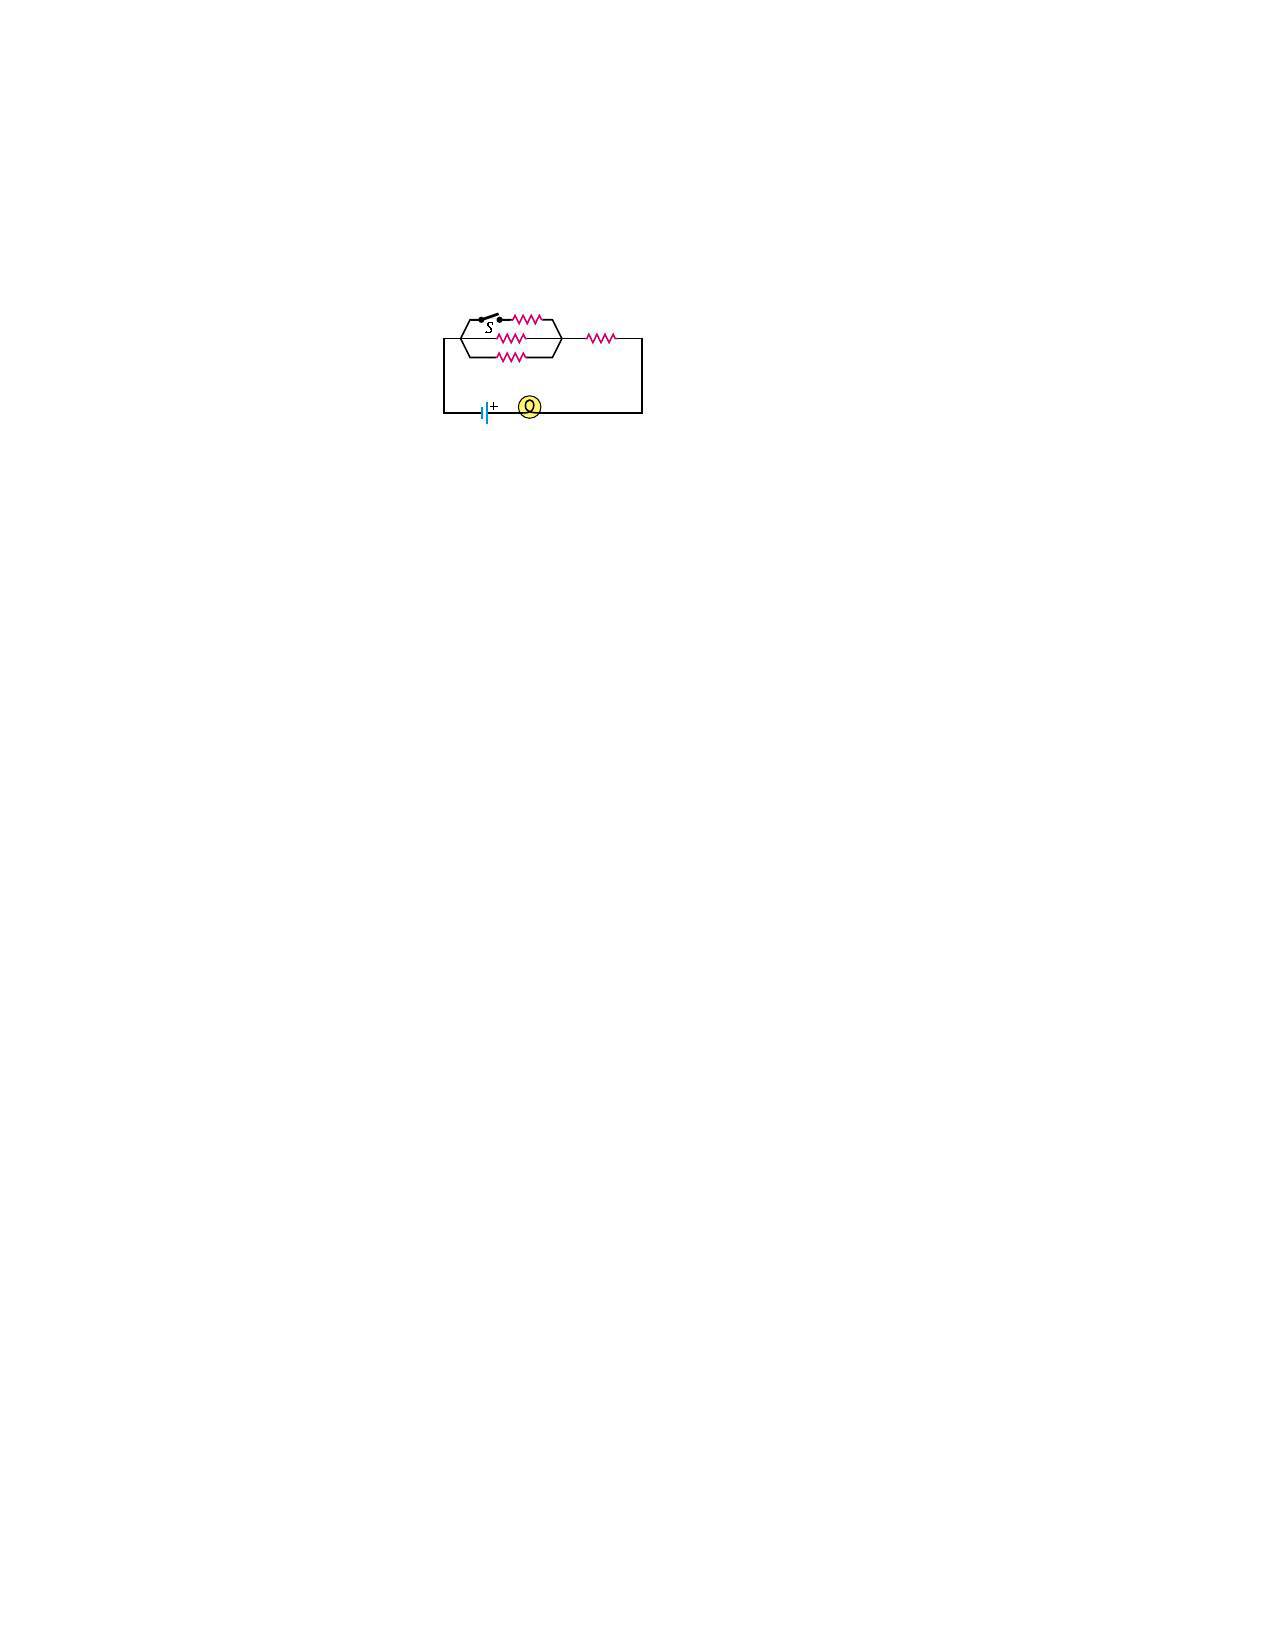
\includegraphics{Q26-9}
\center \textbf{Figure Q26.9}
\end{minipage}

\vfill

\begin{minipage}[l]{0.5\textwidth}
\paragraph{Question 26.18}
\begin{problem}
	Will the capacitors in the circuits shown in \textbf{Fig.~Q26.18} charge at the same rate when the switch $S$ is closed?  If not, in which circuit will the capacitors charge more rapidly?  Explain.
\end{problem}
\end{minipage}%
\hspace{0.05\textwidth}%
\begin{minipage}{0.45\textwidth}
\center {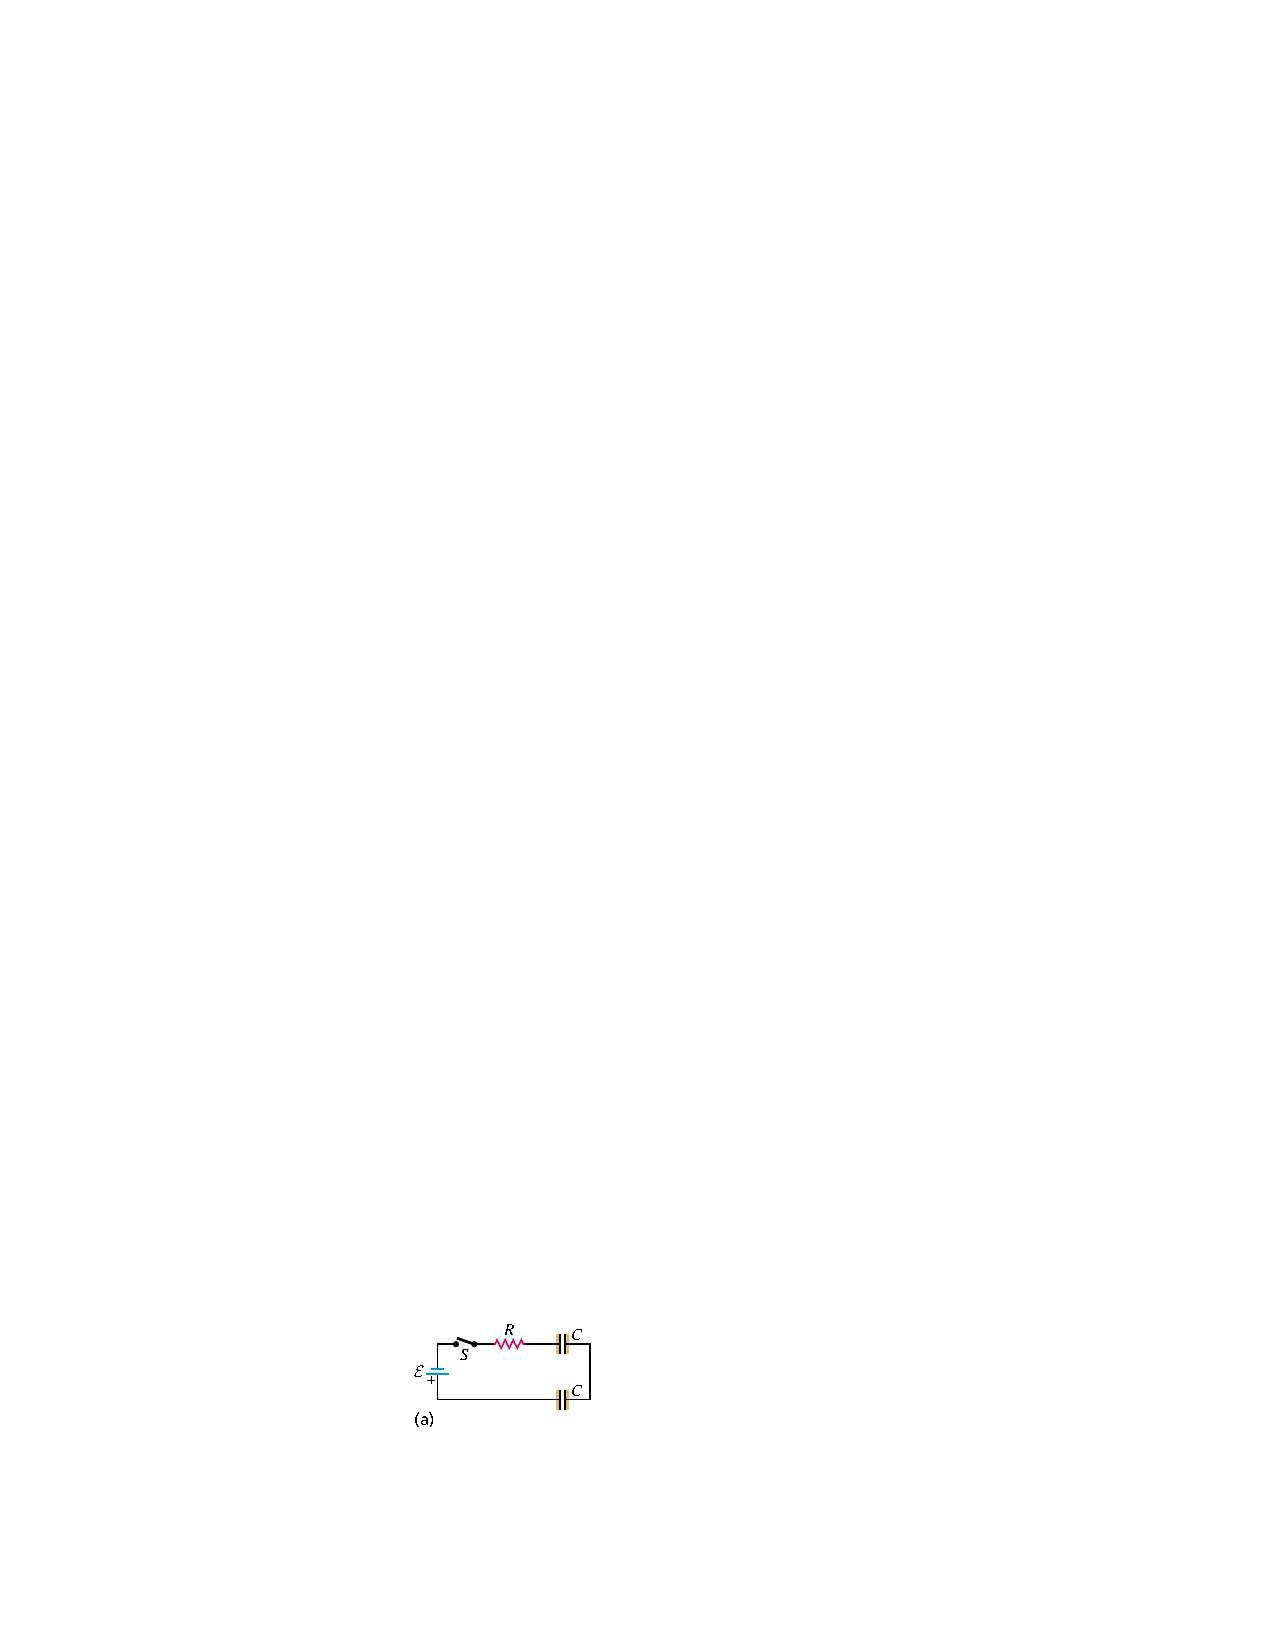
\includegraphics{Q26-18a}
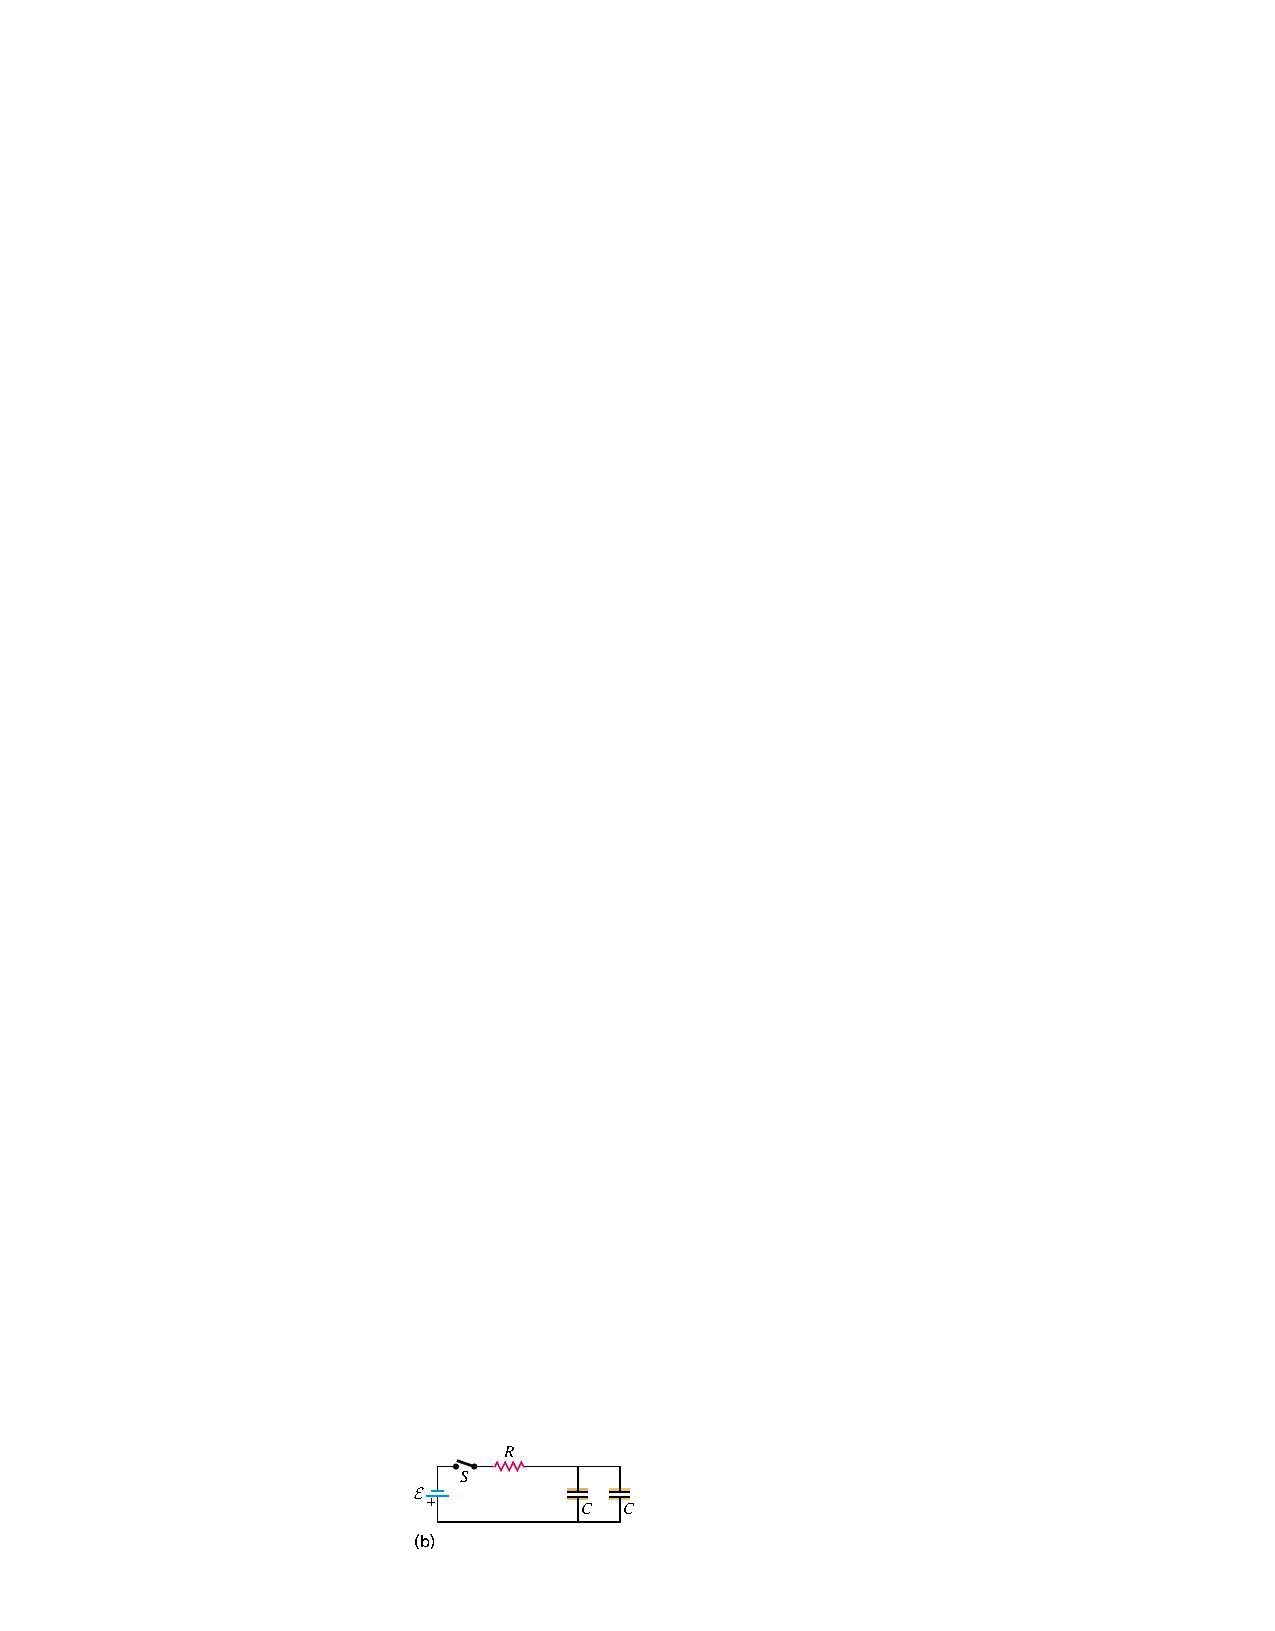
\includegraphics{Q26-18b}}
\center \textbf{Figure Q26.18}
\end{minipage}

\vfill

\end{document}